\subsubsection{Resolver Cuadrados Mínimos usando QR}
Sea A = Q*R la factorización QR de la matriz A mencionada en las secciones anteriores. Entonces, 
\begin{center}
 $\displaystyle \min_{x \in \mathbb{R}^{(n+1)}} \| Ax-b\|^2 = \min_{x \in \mathbb{R}^{(n+1)}} \| Q^tAx-Q^tb \|^2 = \min_{x \in \mathbb{R}^{(n+1)}} \| Rx-Q^tb\|^2$
\end{center}
Como A tiene columnas independientes\footnote{Para más información, referirse a la sección demostraciones}, entonces $R_{i,i} \neq 0 \ \forall i=1,\ldots,n+1$ 
y además {$R_{i,j} = \nobreak 0 \ \forall i=1,\ldots,m; \ j=1,\ldots,i-1 $}. La multiplicacion matriz-vector Rx entonces sería:
\begin{center}
$Rx = \begin{pmatrix}
        R_1x \\
        0
       \end{pmatrix}$ con $R_1 \in \mathbb{R}^{(n+1) \times (n+1)}$ la parte por arriba de la diagonal de $R$.
\end{center}
Además, si reescribimos a $Q^tb$ como:
\begin{center}
$Q^tb = \begin{pmatrix}
        c\\
        d
       \end{pmatrix}$ con $c \in \mathbb{R}^{(n+1) \times (n+1)}$ y $d \in \mathbb{R}^{m-(n+1)}$, problema se reduce a:

$\min_{x \in \mathbb{R}^{(n+1)}} \| Rx-Q^tb\|^2 = \| (R_1x,0)^t -(c,d)^t \|^2 =
\min_{x \in \mathbb{R}^{(n+1)}} \|R_1x-c\|^2+\|d\|^2$

$ \rightarrow \min_{x \in \mathbb{R}^{(n+1)}} \| R_1x-c\|^2 \rightarrow x/ R_1x=c$
\end{center}

\begin{figure}[H] 
\begin{center}
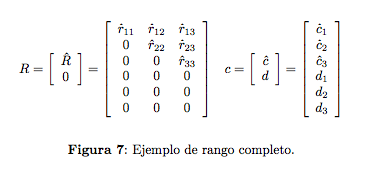
\includegraphics[width=0.6\textwidth]{img/exp-qr.png} 
\end{center}
\end{figure}


El sistema $R_1x=b$ tiene solución dado que $R_1$ es triangular superior con elementos no nulos en la diagonal. Si encontramos el $x$ que sea solución para ese sistema, será el mismo $x$ solución para el problema de Cuadrados Mínimos.





% %%%%%%%%%%%%%%%%%%%%%%%%%%%%%%

% Se plantea el nuevo sistema $Q^t A x = Q^t b$ que equivale a Rx = c, donde $\hat{c}$ son los primeros m elementos de c y d los restantes. El residuo s resulta s = c - Rx, donde los primeros m elementos de s son iguales a $\hat{c}$ - Rx y los restantes a d. De esta forma, el cuadrado del residuo, es decir, lo que se busca minimizar es igual a 

% \begin{center}
% $||$s$||^2_2$ = $||$ $\hat{c} - \hat{R}$x$||^2_2$ + $||$d$||^2_2$
% \end{center}

% Puesto que el segundo termino, d no depende de x, se busca minimizar el primero. Como $\hat{R}$ era no singular, entonces la solucion del sistema $\hat{R}$x = $\hat{c}$ es unica y es la solucion de cuadrados minimos. cabe destacar que el termino es la norma del residuo asociado con solucion obtenida.

